\begin{tikzpicture}[
  declare function={
    gamma(\z) =
    (2.50*sqrt(1/\z)+0.20*(1/\z)^(1.5)+
    0.00*(1/\z)^(2.5)-(174.21*(1/\z)^(3.5))/25920-
    (715.64*(1/\z)^(4.5))/1244160)*exp((-ln(1/\z)-1)*\z);
  },
  declare function={
    gammapdf(\x,\a,\b) = (\b^\a)*\x^(\a-1)*exp(-\b*\x)/gamma(\a);
  }]

  \begin{axis}[
    width=9cm, height=6cm,
    samples=40, no marks, smooth,
    xlabel=$x$, ylabel=$f(x)$,
    xlabel style={at={(1,0)}, anchor=north west},
    ylabel style={at={(0,1)}, anchor=south east},
    legend style={draw=none, fill=none},
    domain=0:22]

    \addplot[black] {gammapdf(x,3,1)};
    \addlegendentry{$\alpha=3, \beta=1$}

    \addplot[blue] {gammapdf(x,8,1)};
    \addlegendentry{$\alpha=8, \beta=1$}

    \addplot[red] {gammapdf(x,8,2)};
    \addlegendentry{$\alpha=8, \beta=2$}

    \node[anchor=east] at (axis description cs: 1,  0.5)
    {$f(x) = \dfrac{\beta^{\alpha}}{\Gamma(\alpha)}\cdot
      x^{\alpha-1} \cdot \text{e}^{-\beta x}$};

  \end{axis}
\end{tikzpicture}

